%% ****** Start of file apstemplate.tex ****** %
%%
%%
%%   This file is part of the APS files in the REVTeX 4 distribution.
%%   Version 4.1r of REVTeX, August 2010
%%
%%
%%   Copyright (c) 2001, 2009, 2010 The American Physical Society.
%%
%%   See the REVTeX 4 README file for restrictions and more information.
%%%
% This is a template for producing manuscripts for use with REVTEX 4.0
% Copy this file to another name and then work on that file.
% That way, you always have this original template file to use.
%
% Group addresses by affiliation; use superscriptaddress for long
% author lists, or if there are many overlapping affiliations.
% For Phys. Rev. appearance, change preprint to twocolumn.
% Choose pra, prb, prc, prd, pre, prl, prstab, prstper, or rmp for journal
%  Add 'draft' option to mark overfull boxes with black boxes
%  Add 'showpacs' option to make PACS codes appear
%  Add 'showkeys' option to make keywords appear





%\documentclass[aps,prl,preprint,superscriptaddress]{revtex4-1}
%\documentclass[aps,prl,reprint,groupedaddress]{revtex4-1}

% You should use BibTeX and apsrev.bst for references
% Choosing a journal automatically selects the correct APS
% BibTeX style file (bst file), so only uncomment the line
% below if necessary.
%\bibliographystyle{apsrev4-1}


% Use the \preprint command to place your local institutional report
% number in the upper righthand corner of the title page in preprint mode.
% Multiple \preprint commands are allowed.
% Use the 'preprintnumbers' class option to override journal defaults
% to display numbers if necessary
%\preprint{}

%Title of paper

\chapter{Comment on ``Phase-Space Approach to Solving the Time-Independent Schr\"{o}dinger Equation"}\label{ch:PRL}

\section{Introduction}
When reproducing the results of the ST paper of \Refc{Shimshovitz2012}, it was determined that certain inaccurate conclusions were drawn. A brief review of \Refc{Shimshovitz2012} is outlined in section \ref{sec:ps} from which is manuscript is a comment on. However, readers are encouraged to have \Refc{Shimshovitz2012} nearby. 

The following content of this chapter is the paper published as \Refc{Brown2015}.


\section{Content of Chapter}


 Shimshovitz and Tannor (ST) \cite{Shimshovitz2012} introduced a periodic von Neumann (vN) basis for solving the Schr\"{o}dinger 
equation. 
%
 Their contribution is important because it outlines ideas that make it possible to prune a vN basis.
  We   point  out that, contrary to statements of ST,  neither their  biorthogonal  pvb basis nor the periodicity of the underlying sinc functions are required
to make  a pruneable basis with which results of similar quality are obtained.  
  The first attempt to use a vN basis \cite{Davis1979} was unsuccessful.  Other approaches to 
exploiting the phase-space locality of 
vN functions  are those of \Refs{Poirier2003,Halverson2012}.

 ST use  vN Gaussians  to contract a 
Fourier grid Hamiltonian \nomenclature{FGH}{Fourier Grid Hamiltonian}(FGH) discrete variable representation (DVR) basis.
  The simultaneous diagonalization basis of \Refs{Dawes2005,Dawes2006} was used in a similar fashion to contract a harmonic basis. 
 ST begin with a pvN\nomenclature{pvN}{Periodic von Neumann} basis, 
%
\begin{equation}\label{PRLeq.1}
\tilde{g}_m\left(x\right) =\sum_{n=1}^{N}\phi_n\left(x\right)g_m\left(x_n\right)
\end{equation}
where  $g_m(x)  $ are  vN Gaussians   and   $\phi_n\left(x\right)$ are  periodic sinc functions centered at 
equally spaced points  $x_n$ and transform  the time-independent Schr\"{o}dinger equation (TISE) in the FGH  basis,
 $\bf{ H   U} = {\bf{UE}}$, 
 
%
%\begin{equation}
%\bf{ H^{sDVR}    U} = {\bf{UE}}
%\end{equation}
to obtain 
\begin{equation}
\bf{G^{\dagger} H G V} = {\bf{S V E}} ~,
\label{PRLpvnunchop}
\end{equation}
where  $G_{ij}=g_j\left(x_i\right)$,  ${\bf{S}}$ = ${\bf{G^{\dagger} G}}$   and ${\bf{U}}$ = ${\bf{GV }}$.   
%
ST propose transforming to a pvb basis, 
\begin{equation}
\bf{S^{-1} G^{\dagger} H G S^{-1}  Z} = {\bf{ S^{-1}    Z E}} ~,
\label{bvnunchop}
\end{equation} 
where ${\bf{Z}}$ = ${\bf{S V }}$. 
Both \Eq{PRLpvnunchop} and \Eq{bvnunchop} are generalized eigenvalue problems of the form 
\begin{equation}
\bf{AY } = {\bf{ BYL}}~.
\label{genform}
\end{equation}  
%
The pruned pvN eigenvalue problem is $\bf{     C^{\dagger}G^{\dagger} H  GCV}  =   \bf{C^{\dagger}SCV \tilde{E}}~$,
%\begin{equation}\label{eq.2}
%\bf{     C^{\dagger}G^{\dagger} H^{sDVR} GCV}  =   \bf{C^{\dagger}SCVE}~, 
%\end{equation}  
 where ${\bf{C}}$ has  $n_k$  diagonal elements equal to   one  and $n_d=N-n_k$  elements equal to zero.  Matrices  playing
 the role of $both$  ${\bf{A }}$  and $ {\bf{ B}}$,  in \Eq{genform}    are chopped.
Pruning  the pvN  basis significantly degrades the accuracy of the energies.   
%
The pruned pvb eigenvalue problem is 
%
\begin{equation}\label{PRLeq.3}
	\bs{C^{\dagger}S^{-1}G^{\dagger} H  GS^{-1}CU}=\bs{C^{\dagger}S^{-1}CU \tilde{E}},
\end{equation}   
and in this basis, it $is$  possible to prune and maintain accuracy!
Again,    
the matrices playing  the role of $both$  ${\bf{A }}$  and $ {\bf{ B}}$  are chopped.   





There is, however,  no need to introduce the pvb basis.   Starting with \Eq{PRLpvnunchop},  moving ${\bf{S}}^{-1}$ to the left and $then $
pruning, one obtains the nonsymmetric eigenvalue problem 
\begin{equation}\label{our}
\bf{C^{\dagger}  S^{-1}  G^{\dagger} H^{DVR} G  CV}={\bf{V  \bar{E}}}.
\end{equation} 
%
It is easier to solve    Eq (\ref{our}) than \Eq{PRLeq.3}   with    iterative eigenvalue solvers  
 because  it is not a generalized eigenvalue problem
(therefore larger systems are accessible).  
%\cite{Bai2000}
%tc this is   Z. Bai, J. Demmel, J. Dongarra, A. Ruhe and H. van der Vorst, editors, 
%Templates for the solution of Algebraic Eigenvalue Problems: A Practical Guide . SIAM, Philadelphia, 2000
%  
For the 1D Morse potential of  Ref. \citenum{Shimshovitz2012},  we compare eigenvalues computed with   \Eq{our}   and \Eq{PRLeq.3},
using  $N=196$ initial basis functions. 
%
In both cases, the error does not 
decrease until about $n_k = 98$.   
 %Thus,  the pvN basis,  truncated using    \Eq{our},  has   most of the advantages of the pvb basis.  
%  The most important idea is to use 
%Gaussians to contract rather than to use them as basis functions.  
%
 \begin{figure}[ht]
 \includegraphics[width=6.5in]{PRL/fig_1ab.eps}%
 \caption[Comparison of different methods for the 22nd eigenvalue of the Morse oscillator]{The error of the 22nd eigenvalue of the Morse oscillator
\label{PRLfig.1} a) Comparison of ST's pvb with the FGH and \Eq{our} with the Colbert and Miller (CM)\cite{Colbert1992} Sinc DVRs. %JB24
   b) Comparison of Hermite (H$_n(x)$) and Legendre (P$_n(x)$) DVRs using \Eq{our} and ST's pvb.}
 \end{figure}
%


According to  ST, the accuracy of the \Eq{PRLeq.3} levels  is due in part  to the
 periodicity of the  sinc DVR.  We have confirmed that with  \Eq{our}, energies obtained with 
non-periodic DVRs \cite{Light2000}  are also accurate; see  Fig. \ref{PRLfig.1}b  for the Morse oscillator of ST. 
 Fig. \ref{PRLfig.1}b is  generated with   vN  functions 
  at $\sqrt{N}$ position values $x_i$ that are  a subset of the    DVR  points. %,  
%
After sending this comment to ST,   we learned that they had done pvb calculations with other DVRs.   \cite{Shimshovitz2014b}  
The fact that both  \Eq{our} and the ST approach work with other DVRs  is clearly incompatible with 
 the assertion  that periodicity is important.  
% 
% When $n_k$ is small the pvN energies are, however, more accurate.  
 %We have  done similar calculations with other potentials.  
%It might be possible to choose the vN parameters  to improve the accuracy.   
%
Knowing that the ST idea of contracting with Gaussians can be applied to other DVRs opens the door to using it to solve many problems
for which      sinc DVRs are not ideal.  
 %Legendre DVRs are well suited to solving problems in polyspherical coordinates.   %Legendre matrix elements of 
%the    polyspherical kinetic energy operator are well known. 
%
% 
%



In summary, it  is not necessary to think in terms of the  pvb basis ST  introduce if the pvN eigenproblem is truncated as in \Eq{our},   and 
 the contraction idea ST use   enables one to use Gaussians to contract any DVR basis. %JB25
%


% If in two-column mode, this environment will change  to single-column
% format so that long equations can be displayed. Use
% sparingly.
%\begin{widetext}
% put long equation here
%\end{widetext}

% figures should be put into the text as floats.
% Use the graphics or graphicx packages (distributed with LaTeX2e)
% and the \includegraphics macro defined in those packages.
% See the LaTeX Graphics Companion by Michel Goosens, Sebastian Rahtz,
% and Frank Mittelbach for instance.
%
% Here is an example of the general form of a figure:
% Fill in the caption in the braces of the \caption{} command. Put the label
% that you will use with \ref{} command in the braces of the \label{} command.
% Use the figure* environment if the figure should span across the
% entire page. There is no need to do explicit centering.

% \begin{figure}[h!]
% \includegraphics[scale=0.4]{fig_1ab.eps}%
% \caption{The error of the 22nd eigenvalue of the Morse oscillator
%\label{fig.1} a) Comparison of ST's pvb  and \Eq{our}.   b) Comparison of three different DVRs using Eq (\ref{our}).}%JBnew added reference to Eq (7)
% \end{figure}

% Surround figure environment with turnpage environment for landscape
% figure
% \begin{turnpage}
% \begin{figure}
% \includegraphics{}%
% \caption{\label{}}
% \end{figure}
% \end{turnpage}

% tables should appear as floats within the text
%
% Here is an example of the general form of a table:
% Fill in the caption in the braces of the \caption{} command. Put the label
% that you will use with \ref{} command in the braces of the \label{} command.
% Insert the column specifiers (l, r, c, d, etc.) in the empty braces of the
% \begin{tabular}{} command.
% The ruledtabular enviroment adds doubled rules to table and sets a
% reasonable default table settings.
% Use the table* environment to get a full-width table in two-column
% Add \usepackage{longtable} and the longtable (or longtable*}
% environment for nicely formatted long tables. Or use the the [H]
% placement option to break a long table (with less control than 
% in longtable).
% \begin{table}%[H] add [H] placement to break table across pages
% \caption{\label{}}
% \begin{ruledtabular}
% \begin{tabular}{}
% Lines of table here ending with \\
% \end{tabular}
% \end{ruledtabular}
% \end{table}

% Surround table environment with turnpage environment for landscape
% table
% \begin{turnpage}
% \begin{table}
% \caption{\label{}}
% \begin{ruledtabular}
% \begin{tabular}{}
% \end{tabular}
% \end{ruledtabular}
% \end{table}
% \end{turnpage}

% Specify following sections are appendices. Use \appendix* if there
% only one appendix.
%\appendix
%\section{}

